\documentclass[12pt,letterpaper]{article}
\usepackage[utf8]{inputenc}
\usepackage[T1]{fontenc}
\usepackage[spanish]{babel}
\usepackage[margin=3cm]{geometry}
\usepackage{graphicx}
\usepackage{enumitem}
\usepackage{amsmath,amssymb}
\usepackage{array}
\usepackage{tikz}
\usepackage[colorlinks=true,linkcolor=black,urlcolor=blue,citecolor=black]{hyperref}
\usepackage{xurl}
\usepackage{titlesec}
\usepackage{parskip}
\usepackage{xcolor}
\titleformat{\section}{\large\bfseries}{\thesection.}{0.5em}{}
\titleformat{\subsection}{\normalsize\bfseries}{\thesubsection.}{0.5em}{}
\emergencystretch=2em
\newcommand{\rub}[1]{\par\medskip\noindent\textbf{#1}\par\nopagebreak}

\begin{document}

\begin{titlepage}
\centering
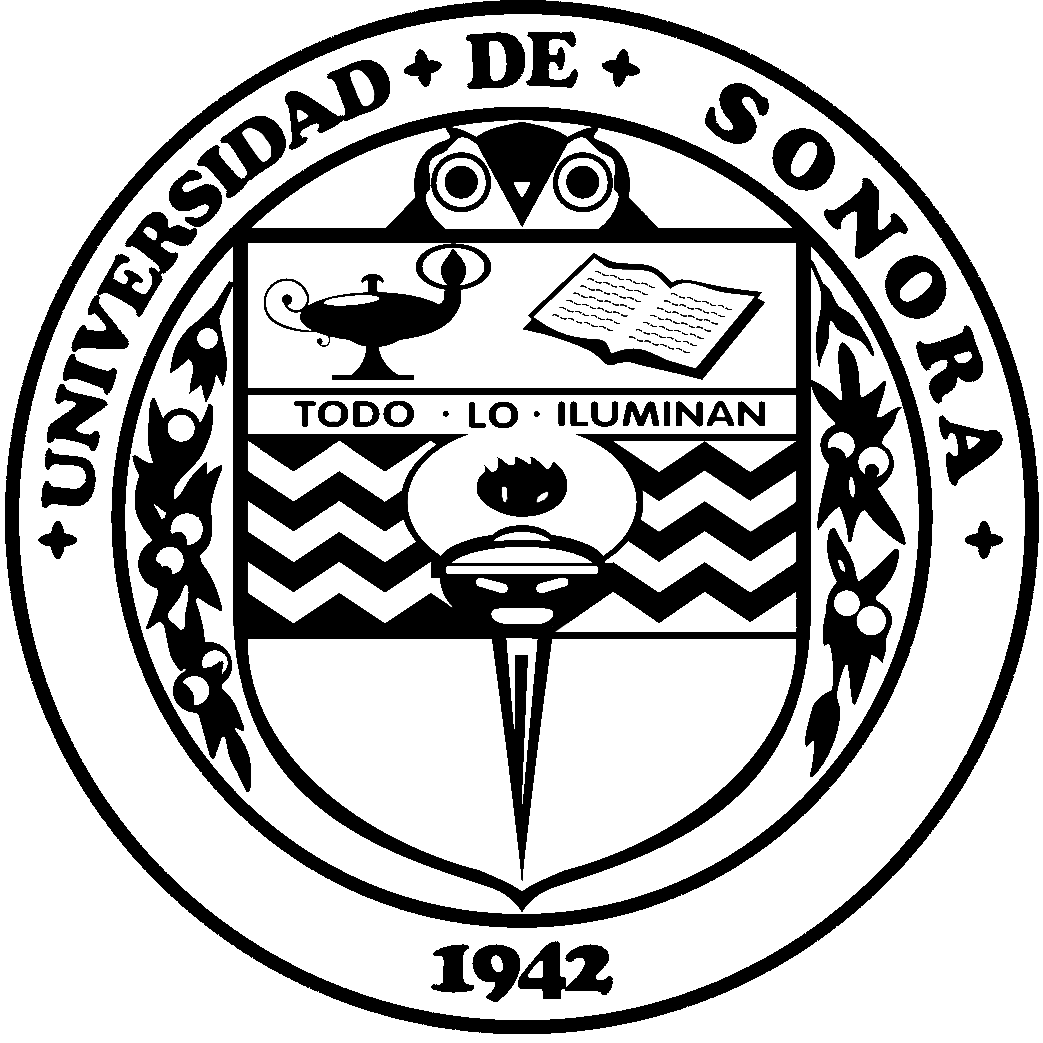
\includegraphics[width=4cm]{escudo.png}\\[0.6cm]
{\Large\bfseries Universidad de Sonora}\\[0.3cm]
{\large Licenciatura en Ciencias de la Computación}\\[1.5cm]
{\LARGE\bfseries Algoritmos de enrutado}\\[0.4cm]
{\large Tarea individual}\\[1.5cm]
\begin{tabular}{rl}
\textbf{Materia:} & Redes de Computadoras I\\
\textbf{Periodo:} & 2026-2\\
\textbf{Profesor:} & Dr. Donald José Rodríguez Úbeda\\
\end{tabular}\\[1.5cm]
{\large\bfseries Alumno}\\[0.3cm]
\begin{tabular}{ll}
Angel Fernando Bórquez Guerrero & Expediente 219208106\\
\end{tabular}\\[1.5cm]
Hermosillo, Sonora \hfill Noviembre de 2026
\end{titlepage}

\tableofcontents
\newpage

\section{Introducción}
La responsabilidad principal de la capa de red es llevar los paquetes desde el origen hasta su destino. En la mayoría de las redes un paquete debe pasar por varios enrutadores antes de llegar, así que alguien tiene que decidir por cuál camino se envía. Los algoritmos que toman esa decisión, y las estructuras de datos que usan, son una pieza central del diseño de la capa de red (Rodríguez Úbeda, 2026; Tanenbaum \& Wetherall, 2011).

Conviene distinguir dos tareas que a veces se confunden. El \textbf{enrutado} es el proceso de construir y mantener las tablas que dicen cuál es el mejor camino hacia cada destino; el \textbf{reenvío} es lo que hace el enrutador con cada paquete: consultar la tabla y mandarlo por la interfaz de salida correspondiente (Kurose \& Ross, 2017). Los algoritmos de este documento pertenecen a la primera tarea.

\subsection{Propiedades deseables y clasificación}
Un buen algoritmo de enrutado debe ser correcto, simple, robusto, estable, justo y óptimo (Rodríguez Úbeda, 2026; Tanenbaum \& Wetherall, 2011). ``Óptimo'' depende de la métrica elegida (número de saltos, distancia, retardo, ancho de banda, costo), y un mismo algoritmo puede combinar varias dándole más peso a una de ellas. Otro criterio importante es la \emph{rapidez de convergencia}: el tiempo que tardan todos los enrutadores en ponerse de acuerdo sobre las mejores rutas después de que un enlace aparece o falla.

Según cómo obtienen la información, los algoritmos se clasifican en:
\begin{itemize}[itemsep=2pt]
\item \textbf{Estáticos} (no adaptativos): todas las rutas se definen de antemano y no cambian por sí solas cuando cambia la red.
\item \textbf{Dinámicos} (adaptativos): los enrutadores intercambian información de manera periódica y ajustan las rutas según el estado actual de la red.
\end{itemize}
Intercambiar información y mantener las tablas tiene un costo, llamado \textbf{sobrecarga}: tráfico de control, memoria y CPU que no se usan para mover datos del usuario (Rodríguez Úbeda, 2026). Esa sobrecarga es una de las comparaciones que se hacen entre los ocho algoritmos descritos a continuación.

\section{Algoritmos de enrutado}

\subsection{Algoritmo de camino más corto}
\rub{En qué consiste}
La red se representa como un grafo: los enrutadores son nodos y los enlaces son aristas con un costo (saltos, distancia, retardo\ldots). El algoritmo calcula, para cada destino, el camino de menor costo total (Tanenbaum \& Wetherall, 2011). Hay dos familias principales:
\begin{itemize}[itemsep=3pt]
\item \textbf{Estado del enlace} (algoritmo de Dijkstra). Cada enrutador conoce la topología completa y el costo de todos los enlaces, y ejecuta el algoritmo de Dijkstra (1959) para obtener el árbol de caminos más cortos con él mismo como raíz. En cada paso se fija el nodo no visitado con menor distancia acumulada y se actualizan las distancias de sus vecinos.
\item \textbf{Vector de distancias} (algoritmo de Bellman-Ford). Cada enrutador solo conoce sus vecinos y mantiene un vector con la distancia a cada destino. Periódicamente intercambia su vector con los vecinos y actualiza $D_x(y) = \min_v \{c(x,v) + D_v(y)\}$ (Bellman, 1958; Kurose \& Ross, 2017).
\end{itemize}

\textbf{Ejemplo.} Considere el grafo de la figura~1 y calcule los caminos más cortos desde $A$ con Dijkstra.
\begin{center}
\begin{tikzpicture}[every node/.style={circle,draw,minimum size=0.75cm,inner sep=0pt,font=\small},
  lab/.style={draw=none,fill=white,inner sep=1pt,font=\footnotesize}]
\node (A) at (0,0) {A};
\node (B) at (2.8,1.4) {B};
\node (C) at (2.8,-1.4) {C};
\node (D) at (5.6,1.4) {D};
\node (E) at (5.6,-1.4) {E};
\draw (A)--node[lab]{2}(B);
\draw (A)--node[lab]{5}(C);
\draw (B)--node[lab]{1}(C);
\draw (B)--node[lab]{4}(D);
\draw (C)--node[lab]{1}(D);
\draw (C)--node[lab]{4}(E);
\draw (D)--node[lab]{2}(E);
\end{tikzpicture}\\[3pt]
{\footnotesize Figura 1. Red de ejemplo; los números son los costos de los enlaces.}
\end{center}
\begin{center}
\small
\begin{tabular}{|c|c|c|c|c|c|}
\hline
\textbf{Paso} & \textbf{Nodo fijado} & $d(B)$ & $d(C)$ & $d(D)$ & $d(E)$\\
\hline
0 & $A$ (0) & 2 & 5 & $\infty$ & $\infty$\\ \hline
1 & $B$ (2) & -- & 3 & 6 & $\infty$\\ \hline
2 & $C$ (3) & -- & -- & 4 & 7\\ \hline
3 & $D$ (4) & -- & -- & -- & 6\\ \hline
4 & $E$ (6) & -- & -- & -- & --\\ \hline
\end{tabular}\\[3pt]
{\footnotesize Tabla 1. Ejecución de Dijkstra desde $A$.}
\end{center}
Resultado: $A\to B$ cuesta 2 (directo); $A\to C$ cuesta 3 (por $B$, mejor que el enlace directo de costo 5); $A\to D$ cuesta 4 (por $B$ y $C$); $A\to E$ cuesta 6 (por $B$, $C$ y $D$).

\rub{Ventajas}
\begin{itemize}[itemsep=2pt]
\item Produce rutas óptimas respecto a la métrica elegida.
\item Estado del enlace: converge rápido y de forma estable, porque cada enrutador tiene la misma visión de la red.
\item Vector de distancias: es simple de implementar y requiere poca memoria y cálculo.
\end{itemize}
\rub{Desventajas}
\begin{itemize}[itemsep=2pt]
\item Estado del enlace: cada enrutador debe almacenar toda la topología y repartir las actualizaciones a todos, lo que consume memoria, CPU y ancho de banda; escala mal sin jerarquía.
\item Vector de distancias: converge lentamente y sufre el problema de la ``cuenta al infinito'': las malas noticias (un enlace caído) se propagan despacio y pueden formar bucles temporales (Tanenbaum \& Wetherall, 2011).
\end{itemize}
\rub{Ejemplos de uso}
\begin{itemize}[itemsep=2pt]
\item \textbf{OSPF} (Moy, 1998) e \textbf{IS-IS} (Callon, 1990) son protocolos de estado del enlace que usan Dijkstra; se emplean dentro de redes de operadores y empresas.
\item \textbf{RIP} (Hedrick, 1988; Malkin, 1998) es un protocolo de vector de distancias con el número de saltos como métrica; su límite es de 15 saltos y se usa en redes pequeñas.
\end{itemize}

\subsection{Encaminamiento de camino múltiple}
\rub{En qué consiste}
En lugar de elegir una sola ruta por destino, el enrutador guarda varias y reparte el tráfico entre ellas. La variante más extendida es \emph{Equal-Cost Multi-Path} (ECMP): cuando hay varios caminos de igual costo, se usan todos. Para no desordenar los paquetes de una misma conexión, el reparto se hace por flujo: se calcula una función hash sobre campos del encabezado (direcciones y puertos) y el resultado determina el siguiente salto. El RFC 2992 analiza tres formas de elegirlo: módulo~$N$, umbral de hash (\emph{hash-threshold}) y peso aleatorio más alto; en el análisis, la elección por módulo cambia de ruta a la fracción $(N-1)/N$ de los flujos cuando cambia el número de rutas, el umbral de hash entre $1/4$ y $1/2$, y el peso aleatorio más alto solo $1/N$, aunque con mayor costo de cálculo (Hopps, 2000).
\rub{Ventajas}
\begin{itemize}[itemsep=2pt]
\item Aprovecha todos los enlaces disponibles, con más ancho de banda total y menos congestión.
\item Si una ruta falla, el tráfico pasa a las restantes sin esperar a recalcular desde cero, lo que mejora la tolerancia a fallas.
\end{itemize}
\rub{Desventajas}
\begin{itemize}[itemsep=2pt]
\item Requiere más memoria en las tablas y funciones de reparto más complejas.
\item El reparto por hash puede ser desigual: pocos flujos muy grandes pueden caer en el mismo camino.
\item Cuando cambia el conjunto de rutas, parte de los flujos cambia de camino, lo que puede reordenar paquetes y afectar a TCP (Hopps, 2000).
\end{itemize}
\rub{Ejemplos de uso}
\begin{itemize}[itemsep=2pt]
\item OSPF e IS-IS pueden instalar varias rutas de igual costo (Moy, 1998).
\item Las redes de centros de datos con topología \emph{fat-tree} tienen muchos caminos de igual costo entre servidores, que se aprovechan con ECMP o variantes (Al-Fares et al., 2008).
\end{itemize}

\subsection{Encaminamiento por gestión centralizada}
\rub{En qué consiste}
Un elemento central (el centro de control de enrutado) recoge el estado de toda la red, calcula las rutas óptimas y las distribuye a los enrutadores, que solo ejecutan el reenvío. En la práctica actual esta idea aparece en las redes definidas por software (SDN), donde un controlador separa el plano de control del de datos y programa los conmutadores, por ejemplo con OpenFlow (McKeown et al., 2008; Kreutz et al., 2015).
\rub{Ventajas}
\begin{itemize}[itemsep=2pt]
\item Visión global de la red, de modo que puede optimizar el tráfico en conjunto y no solo ruta por ruta.
\item Los enrutadores son más sencillos: no ejecutan protocolos de enrutado complejos.
\item Es fácil cambiar la política desde un solo lugar.
\end{itemize}
\rub{Desventajas}
\begin{itemize}[itemsep=2pt]
\item El controlador es un punto único de falla y un posible cuello de botella; se suele replicar.
\item Los enrutadores dependen del enlace con el controlador, y la reacción a un fallo incluye el retardo de ida y vuelta.
\item El controlador debe soportar el tamaño de toda la red.
\end{itemize}
\rub{Ejemplos de uso}
\begin{itemize}[itemsep=2pt]
\item \textbf{B4} de Google, la red que interconecta sus centros de datos: un servicio centralizado de ingeniería de tráfico reparte el ancho de banda entre aplicaciones según su prioridad y lleva los enlaces ``cerca del 100~\%'' de utilización, frente al 30--40~\% típico de otras redes de área amplia. Además, si se desactiva, la red regresa al enrutado de camino más corto (Jain et al., 2013).
\end{itemize}

\subsection{Encaminamiento aislado}
\rub{En qué consiste}
Cada nodo decide por sí solo, usando únicamente la información local que tiene (lo que ve llegar o el estado de sus propias colas), sin intercambiar información de enrutado con otros nodos ni conocer la topología. Los tres algoritmos siguientes (patata caliente, retroaprendizaje e inundación) son ejemplos de esta clase y se describen por separado.
\rub{Ventajas}
\begin{itemize}[itemsep=2pt]
\item Sin sobrecarga de tráfico de control ni protocolos de intercambio.
\item Implementación simple y muy robusta, porque no hay información global que pueda quedar desactualizada.
\end{itemize}
\rub{Desventajas}
\begin{itemize}[itemsep=2pt]
\item Sin información global las decisiones suelen ser subóptimas: los paquetes pueden dar rodeos o llegar duplicados.
\item Rendimiento difícil de predecir en redes grandes.
\end{itemize}
\rub{Ejemplos de uso}
\begin{itemize}[itemsep=2pt]
\item Los tres algoritmos siguientes: patata caliente, retroaprendizaje e inundación.
\end{itemize}

\subsection{Algoritmo de ``patata caliente'' (\emph{hot potato})}
\rub{En qué consiste}
El nodo intenta deshacerse del paquete lo antes posible: lo coloca en la cola de salida más corta (la menos ocupada), sin considerar el destino. Fue propuesto por Paul Baran en el diseño de las redes de comunicaciones distribuidas, donde la idea era que el paquete siguiera avanzando aunque no fuera por el mejor camino (Baran, 1964).

El mismo nombre se usa en BGP para la regla de \emph{salida temprana}: entre varias rutas igualmente buenas hacia un destino externo, el enrutador elige la que sale de su sistema autónomo por el punto más cercano, es decir, con menor costo dentro de la red (Teixeira et al., 2004).
\rub{Ventajas}
\begin{itemize}[itemsep=2pt]
\item Muy simple y rápido: no necesita tablas ni intercambiar información.
\item Reparte la carga: los paquetes se alejan de las colas largas, lo que reduce la congestión local.
\item En BGP, limita el ancho de banda que se consume dentro de la red propia, pues entrega el tráfico al siguiente sistema autónomo lo antes posible (Teixeira et al., 2004).
\end{itemize}
\rub{Desventajas}
\begin{itemize}[itemsep=2pt]
\item Los caminos son largos e ineficientes, y un paquete puede dar vueltas sin acercarse al destino.
\item Los paquetes de un mismo mensaje pueden llegar desordenados.
\item En BGP, un cambio de costo interno puede cambiar el punto de salida, causar bucles transitorios, desplazar mucho tráfico a otras rutas y generar actualizaciones BGP visibles para otras redes (Teixeira et al., 2004).
\end{itemize}
\rub{Ejemplos de uso}
\begin{itemize}[itemsep=2pt]
\item Propuesta original de Baran (1964) para redes distribuidas resistentes a fallos.
\item Regla de salida temprana en el enrutado entre sistemas autónomos con BGP (Teixeira et al., 2004; Rekhter et al., 2006).
\end{itemize}

\subsection{Algoritmo de retroaprendizaje (\emph{backward learning})}
\rub{En qué consiste}
El nodo aprende la topología observando el tráfico que le llega: cada vez que recibe una trama con dirección de origen $S$ por la interfaz $i$, anota que $S$ se alcanza a través de $i$. Al recibir una trama para el destino $D$, consulta la tabla: si $D$ ya fue aprendido, la envía solo por esa interfaz; si no, la reenvía por todas las demás (inundación). Para tolerar cambios, las entradas caducan si no se refrescan (Tanenbaum \& Wetherall, 2011).
\rub{Ventajas}
\begin{itemize}[itemsep=2pt]
\item Funciona sin configuración y sin protocolo de intercambio de rutas.
\item Se adapta solo a que una máquina cambie de lugar, porque el siguiente tráfico actualiza la entrada.
\item Con el tiempo reduce la inundación: el tráfico se envía solo por donde hace falta.
\end{itemize}
\rub{Desventajas}
\begin{itemize}[itemsep=2pt]
\item Solo aprende por donde llegó el tráfico, así que al principio (o para destinos que nunca envían) debe inundar.
\item Con ciclos en la topología, las tramas pueden circular indefinidamente; por eso se acompaña de un protocolo de árbol de expansión (Perlman, 1985).
\item La tabla es finita: un atacante puede llenarla con direcciones falsas y obligar al conmutador a inundar.
\end{itemize}
\rub{Ejemplos de uso}
\begin{itemize}[itemsep=2pt]
\item Los puentes transparentes y los conmutadores Ethernet (IEEE 802.1D) aprenden las direcciones MAC de esta manera (IEEE, 2004; Tanenbaum \& Wetherall, 2011).
\end{itemize}

\subsection{Algoritmo de inundación (\emph{flooding})}
\rub{En qué consiste}
Cada paquete que llega a un nodo se reenvía por todas las interfaces, excepto por la que llegó. Como esto genera una cantidad enorme de duplicados, se limitan con mecanismos como un contador de saltos que disminuye en cada nodo y descarta el paquete en cero, números de secuencia para no reenviar dos veces el mismo paquete, o la inundación selectiva, que solo reenvía hacia la dirección general del destino (Tanenbaum \& Wetherall, 2011).
\rub{Ventajas}
\begin{itemize}[itemsep=2pt]
\item Es muy robusto: mientras exista algún camino entre origen y destino, el paquete llegará.
\item Siempre encuentra el camino más corto, pues una de las copias lo recorre.
\item No necesita conocer la topología ni mantener tablas.
\item Es adecuado para difundir información a todos los nodos.
\end{itemize}
\rub{Desventajas}
\begin{itemize}[itemsep=2pt]
\item Genera un número muy grande de paquetes duplicados y desperdicia ancho de banda.
\item Sin control (contador de saltos o números de secuencia) puede saturar la red.
\end{itemize}
\rub{Ejemplos de uso}
\begin{itemize}[itemsep=2pt]
\item Los protocolos de estado del enlace reparten sus anuncios por inundación: OSPF inunda los anuncios de estado de enlace (LSA) a todos los enrutadores del área (Moy, 1998).
\item En redes \emph{ad hoc}, AODV descubre rutas inundando solicitudes de ruta (Perkins et al., 2003).
\item Los conmutadores Ethernet inundan las tramas con destino desconocido (ver retroaprendizaje).
\end{itemize}

\subsection{Técnica de encaminamiento jerárquico}
\rub{En qué consiste}
En redes muy grandes una tabla con todos los destinos sería enorme. Con la jerarquía, los enrutadores se agrupan en regiones: cada enrutador conoce la topología detallada de su región y solo una visión resumida de las demás, de modo que su tabla tiene entradas para los enrutadores de su región y para las otras regiones como un todo (Kleinrock \& Kamoun, 1977; Tanenbaum \& Wetherall, 2011). Se puede aplicar en varios niveles (regiones, grupos de regiones, \ldots).
\rub{Ventajas}
\begin{itemize}[itemsep=2pt]
\item Las tablas son mucho más pequeñas, lo que reduce memoria y tiempo de cálculo.
\item Menos tráfico de actualización: un cambio dentro de una región no se propaga a las demás.
\item Escala a redes del tamaño de Internet y permite que cada organización administre su región.
\end{itemize}
\rub{Desventajas}
\begin{itemize}[itemsep=2pt]
\item Las rutas pueden no ser las más cortas, porque al resumir una región se pierde detalle (Kleinrock \& Kamoun, 1977).
\item Requiere planear la división en regiones y es más complicada de configurar.
\end{itemize}
\rub{Ejemplos de uso}
\begin{itemize}[itemsep=2pt]
\item Internet: dentro de cada sistema autónomo se usa un protocolo interno (OSPF, IS-IS, RIP) y entre sistemas autónomos se usa BGP (Rekhter et al., 2006).
\item OSPF divide una red en áreas conectadas a un área troncal (Moy, 1998); IS-IS usa niveles de manera parecida (Callon, 1990).
\end{itemize}

\section{Comparación}
\begin{center}
\small
\renewcommand{\arraystretch}{1.15}
\begin{tabular}{|>{\raggedright\arraybackslash}p{3.2cm}|>{\raggedright\arraybackslash}p{3.6cm}|>{\raggedright\arraybackslash}p{3.6cm}|>{\raggedright\arraybackslash}p{2.9cm}|}
\hline
\textbf{Algoritmo} & \textbf{Principal ventaja} & \textbf{Principal desventaja} & \textbf{Ejemplo}\\
\hline
Camino más corto & Rutas óptimas & Sobrecarga (estado del enlace) o convergencia lenta (vector de distancias) & OSPF, IS-IS, RIP\\ \hline
Camino múltiple & Usa varios caminos a la vez & Posible reordenamiento y reparto desigual & ECMP en centros de datos\\ \hline
Gestión centralizada & Visión global de la red & Punto único de falla & SDN, B4 de Google\\ \hline
Aislado & Sin tráfico de control & Rutas subóptimas & Los tres siguientes\\ \hline
Patata caliente & Muy simple; evita colas largas & Caminos largos y desorden & Baran; salida temprana en BGP\\ \hline
Retroaprendizaje & Sin configuración & Necesita inundar al inicio; requiere árbol de expansión & Conmutadores Ethernet\\ \hline
Inundación & Muy robusto; encuentra el camino más corto & Muchos paquetes duplicados & Anuncios de OSPF; AODV\\ \hline
Jerárquico & Tablas pequeñas, escala bien & Rutas no siempre las más cortas & Sistemas autónomos y áreas OSPF\\ \hline
\end{tabular}\\[3pt]
{\footnotesize Tabla 2. Comparación de los algoritmos de enrutado.}
\end{center}

\section{Conclusiones}
No existe un algoritmo de enrutado mejor en todos los casos: cada uno intercambia exactitud de las rutas contra sobrecarga y simplicidad. El camino más corto da rutas óptimas a cambio de intercambiar información; la inundación y la patata caliente no necesitan casi nada, pero desperdician recursos; el encaminamiento jerárquico permite que las redes grandes funcionen al precio de rutas ligeramente peores, y el camino múltiple y la gestión centralizada buscan aprovechar mejor la capacidad de la red. En la práctica se combinan: por ejemplo, Internet usa jerarquía con protocolos de estado del enlace y de vector de rutas, ECMP para repartir carga, inundación para distribuir los anuncios y, en las redes de grandes centros de datos, controladores centralizados.

\newpage
\section*{Referencias}
\addcontentsline{toc}{section}{Referencias}
\begin{itemize}[leftmargin=1.5em,itemsep=7pt]
\item[] Al-Fares, M., Loukissas, A., \& Vahdat, A. (2008). A scalable, commodity data center network architecture. \emph{ACM SIGCOMM Computer Communication Review, 38}(4), 63--74.
\item[] Baran, P. (1964). On distributed communications networks. \emph{IEEE Transactions on Communications Systems, 12}(1), 1--9.
\item[] Bellman, R. (1958). On a routing problem. \emph{Quarterly of Applied Mathematics, 16}(1), 87--90.
\item[] Callon, R. (1990). \emph{RFC 1195: Use of OSI IS-IS for routing in TCP/IP and dual environments}. Internet Engineering Task Force.
\item[] Dijkstra, E. W. (1959). A note on two problems in connexion with graphs. \emph{Numerische Mathematik, 1}(1), 269--271.
\item[] Hedrick, C. (1988). \emph{RFC 1058: Routing Information Protocol}. Internet Engineering Task Force.
\item[] Hopps, C. (2000). \emph{RFC 2992: Analysis of an equal-cost multi-path algorithm}. Internet Engineering Task Force. \url{https://www.rfc-editor.org/rfc/rfc2992}
\item[] Institute of Electrical and Electronics Engineers. (2004). \emph{IEEE Std 802.1D-2004: IEEE standard for local and metropolitan area networks: Media access control (MAC) bridges}. IEEE.
\item[] Jain, S., Kumar, A., Mandal, S., Ong, J., Poutievski, L., Singh, A., \ldots{} Vahdat, A. (2013). B4: Experience with a globally-deployed software defined WAN. \emph{ACM SIGCOMM Computer Communication Review, 43}(4), 3--14.
\item[] Kleinrock, L., \& Kamoun, F. (1977). Hierarchical routing for large networks: Performance evaluation and optimization. \emph{Computer Networks, 1}(3), 155--174.
\item[] Kreutz, D., Ramos, F. M. V., Veríssimo, P. E., Rothenberg, C. E., Azodolmolky, S., \& Uhlig, S. (2015). Software-defined networking: A comprehensive survey. \emph{Proceedings of the IEEE, 103}(1), 14--76.
\item[] Kurose, J. F., \& Ross, K. W. (2017). \emph{Computer networking: A top-down approach} (7.ª ed.). Pearson.
\item[] Malkin, G. (1998). \emph{RFC 2453: RIP version 2}. Internet Engineering Task Force.
\item[] McKeown, N., Anderson, T., Balakrishnan, H., Parulkar, G., Peterson, L., Rexford, J., \ldots{} Turner, J. (2008). OpenFlow: Enabling innovation in campus networks. \emph{ACM SIGCOMM Computer Communication Review, 38}(2), 69--74.
\item[] Moy, J. (1998). \emph{RFC 2328: OSPF version 2}. Internet Engineering Task Force.
\item[] Perkins, C., Belding-Royer, E., \& Das, S. (2003). \emph{RFC 3561: Ad hoc on-demand distance vector (AODV) routing}. Internet Engineering Task Force.
\item[] Perlman, R. (1985). An algorithm for distributed computation of a spanning tree in an extended LAN. \emph{ACM SIGCOMM Computer Communication Review, 15}(4), 44--53.
\item[] Rekhter, Y., Li, T., \& Hares, S. (Eds.). (2006). \emph{RFC 4271: A border gateway protocol 4 (BGP-4)}. Internet Engineering Task Force.
\item[] Rodríguez Úbeda, D. J. (2026). \emph{Unidad V: Algoritmos de enrutado} [Presentación de diapositivas]. Redes de Computadoras I, Universidad de Sonora.
\item[] Tanenbaum, A. S., \& Wetherall, D. J. (2011). \emph{Computer networks} (5.ª ed.). Prentice Hall.
\item[] Teixeira, R., Shaikh, A., Griffin, T., \& Rexford, J. (2004). Dynamics of hot-potato routing in IP networks. En \emph{Proceedings of ACM SIGMETRICS/Performance 2004}. ACM.
\end{itemize}
\end{document}
